\toclesssection{SCP 017 - Shadow Person}
\addcontentsline{toc}{section}{SCP 017 - Shadow Person}

\textbf{Item \#:} SCP-017

\textbf{Object Class:} Keter

\begin{figure}[h]
\begin{center}
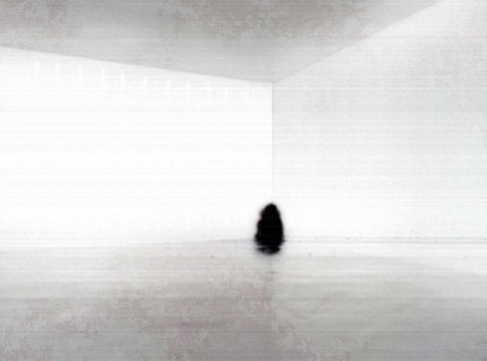
\includegraphics[scale=0.5]{scp/017.jpg}
\linebreak File footage of SCP-017
\end{center}
\end{figure}

\textbf{Special Containment Procedures:} SCP-017 is contained in an acrylic glass cage, 100 cm by 50 cm by 50 cm, centrally suspended in a concrete room measuring 6 m by 6 m by 4 m. Attached to the walls, ceiling, and floor of the room are high-intensity arc lamp spotlights pointed directly at the acrylic cage, to ensure that SCP-017 is constantly exposed to light from every angle. Personnel assigned to the SCP-017 control room are to monitor the functionality of the spotlights and the emergency generator system and call for maintenance immediately upon knowledge of a burnt-out lamp or an issue with the generator.

The only circumstance under which personnel are allowed entrance is to replace lamps. Personnel entering the room are required to wear the designated full-body reflective suits, and must be cautioned not to step in front of functional spotlights.

\textbf{Description:} SCP-017 is a humanoid figure approximately 80 centimeters in height, anatomically similar to a small child, but with no discernible identifying features. SCP-017 seems composed of a shadowy, smoke-like shroud. No attempt to find any object beneath the shroud has been successful, but the possibility has not been ruled out.
\newpage
SCP-017's reaction to shadows cast upon it is immediate and swift. SCP-017 leaps at the object casting the shadow and completely encloses it in its shroud, whereupon it returns to its normal size, leaving no trace of the object behind.

\textbf{Additional Notes:} Personnel with BETA clearance or higher should see also document \#017-1.